\chapter{Rover Software}
\section{Configuring Raspberry Pi}
\paragraph{}The first step of configuration is installation of the Raspberry OS onto the provided SD card. During installation process connection to the phone’s Wi-Fi hotspot was preconfigured, as connecting to eduroam needed more steps in the system itself. For remote terminal access, SSH was enabled.
Before the whole rover was assembled, tasks on the  Raspberry Pi were performed with the help of an external monitor and micro USB power block. When the whole system was assembled, rover's batteries powered the circuit. 
\paragraph{}SSH protocol was used to enable the necessary interfaces for the rover, as well as the built-in Virtual Network Computing (VNC) server. VNC is a software that allows remote control of the Raspberry Pi’s desktop without other peripherals. 

\subsection{Connection via SSH}
\paragraph{}Both Raspberry Pi and the computer must be connected to the same network.The host is formed by the username and the IP address of the board. 
\paragraph{} The most convenient way to utilize SSH connection is via an additional client program. For this reason, MobaXTerm application was used. MobaXterm provides a user-friendly interface that simplifies remote access to the Raspberry Pi \cite{mobxterm:main}. Additionally, MobaXterm supports SFTP, enabling easy file transfer between the local computer and the Raspberry Pi via the built-in file explorer. Another helpful feature is a build-in text editor that is more efficient during coding. 

\subsection{Connection to eduroam network}
\paragraph{} Connection to eduroam on Linux could be done through a configurator program or manually. Due to the performance issues related to the currently installed on Raspberry Pi web browser, our team had to find alternatives that didn’t rely on it, such as downloading the eduroam configuration script externally and then uploading it to the board via mobaXTerm. The network configuration was done manually. File \lstinline|wpa_supplicant.conf| holds the information of all known networks. The following adjustments were made in this file: 

\begin{lstlisting}
 network={
        ssid="eduroam"
        scan_ssid=1
        key_mgmt=WPA-EAP
        eap=PEAP
        identity="youridentity@thm.de"
        password="yourpassword"
        phase1="peaplabel=0"
        phase2="auth=MSCHAPV2"
}
\end{lstlisting}

\paragraph{}Where \lstinline|youridentity| would be substituted with any valid THM user identifier and \lstinline|yourpassword| would be the corresponding user’s net password.
After a reboot, Raspberry Pi was connected successfully as shown on figure \ref{fig:edu_connect}:
\begin{figure}[h]
     \vspace{0.4cm}
     \centering
     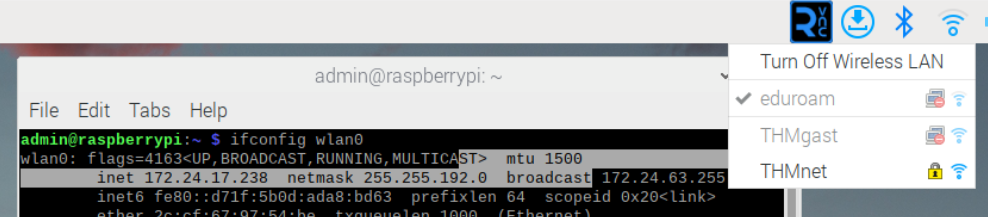
\includegraphics[width=0.9\linewidth]{Hauptkapitel/Pictures/edu_connect.png}
     \caption{Connection to eduroam}
     \label{fig:edu_connect}
 \end{figure}

\section{4tronix scripts for the rover}
\paragraph{}4tronix provides a ready to use scripts for the rover. Most of them are for testing and calibration of the hardware \cite{rover.prog:doc,}. The scripts were obtained from official site of 4tronix via the command \lstinline|wget https://4tronix.co.uk/rover.sh -O rover.sh|. \lstinline|rover.sh| script installs Python libraries and scripts. Their functionality is described in the following table \ref{tab:rv_scripts}.
\newpage
\begin{table}[h]
    \centering
    \begin{longtable}{|l|p{10cm}|}
        \hline
        \textbf{Script} & \textbf{Functionality}\\
        \hline
        \lstinline|calibrateServos.py| & Ensures that the wheels are all pointing in the correct direction. Used for testing servos. \\
        \hline
        \lstinline|rover.py| & The main library module. Consists of functions to manipulate hardware. \\
        \hline
        \lstinline|motorTest.py| & Demonstrates driving the motors. \\
        \hline
        \lstinline|servoTest.py| & Demonstrates controlling the servos. The second script for testing servos. \\
        \hline
        \lstinline|ledTest.py| & Flashes all LEDs through Red, Green, Blue and White. \\
        \hline
        \lstinline|sonarTest.py| & Shows the distance in cm for an obstacle using the ultrasonic distance sensor mounted on the mast head. \\
        \hline
        \lstinline|keypad.py| & Shows the numeric value of each key pressed on the optional keypad. \\
        \hline
        \lstinline|driveRover.py| & Basic driving program using the arrow keys to steer and move. \\
        \hline
    \end{longtable}
    \caption{Scripts provided by 4tronix}
    \label{tab:rv_scripts}
\end{table}
\vspace{-10mm}
\paragraph{}As it is mentioned in the table \ref{tab:rv_scripts},  \lstinline|rover.py| is the core component for a development. Based on this library a script \lstinline|driveRovermqtt.py| was developed to control the rover. 

\section{\lstinline|driveRovermqtt.py| script}
\paragraph{}\lstinline|driveRovermqtt.py| script contain main functionality of the rover. It also controls communication with MQTT broker. Communication side of the project will be explained in later chapters.

\subsection{Rover configuration and motion control}
\subsection{Rover hardware configuration}
\paragraph{} The following variables allow to configure the rover. 
\begin{lstlisting}[style=courier12]
# Rover Configuration
SERVO_FRONT_LEFT = 9
SERVO_REAR_LEFT = 11
SERVO_FRONT_RIGHT = 15
SERVO_REAR_RIGHT = 13
SERVO_MAST = 6
SERVO_TEMPHUM = 25

DEFAULT_SPEED = 60
INACTIVITY_TIMEOUT = 10  # Stop rover if no command received in 10 sec.
DEGREE_STEP = 15  # Mast rotation step
RECONNECT_DELAY = 5  # Delay before reconnecting MQTT after a failure
TEMPERATURE_HIGH_THRESHOLD = 30 #Upper temperature threshold
TEMPERATURE_LOW_THRESHOLD = 0 #Lower temperature threshold
HUMIDITY_THRESHOLD = 80
\end{lstlisting}
\vspace{-5mm}
\paragraph{} Variables \lstinline|RECONNECT_DELAY| and \lstinline|INACTIVITY_TIMEOUT| are important safety features. They help to deal with lost connection. Variables \lstinline|TEMPERATURE_HIGH_THRESHOLD|,\lstinline|TEMPERATURE_LOW_THRESHOLD| and \lstinline|HUMIDITY_THRESHOLD| are used for the functionality of the DHT 22 sensor.
\paragraph{} The main function for controlling the movement is \lstinline|move_rover()|.
\begin{lstlisting}[style=courier12]
def move_rover(key):
    global speed
    global client
    actions = {
        'w': move_forward,
        's': move_reverse,
        'd': turn_right,
        'a': turn_left,
        ' ': reset_servos,
        'q': lambda: rotate_mast(1),
        'e': lambda: rotate_mast(-1),
        'b': stop_rover,
        'p': lambda: publish_photo(client), #Photo task is run on a background thread to prevent stopping the system
        't': taylorSwiftmode,
    }
    if key in actions:
        actions[key]()
    elif key in {'.', '>'}:
        speed = min(100, speed + 10)
        print(f"Speed increased to {speed}")
    elif key in {',', '<'}:
        speed = max(0, speed - 10)
        print(f"Speed decreased to {speed}")
    else:
        print(f"[WARNING] Unknown command received: {key}")
\end{lstlisting}
\paragraph{}The function gets commands from an MQTT client stream and orchestrates the movement. Movement functions are based on the methods from \lstinline|rover.py| library.   

\subsection{MQTT client}
\paragraph{} For the MQTT implementation, the library \lstinline|paho.mqtt.client| was used. The rover connects to the MQTT broker during an initialization process through standard methods of \lstinline|paho.mqtt.client|. In addition to that, customized functions were developed.
\paragraph{} The functions to handle MQTT messages and communication are represented in a table \ref{tab:func_mqtt}.
\begin{table}[h]
    \centering
    \begin{longtable}{|l|p{10cm}|}
        \hline
        \textbf{Function} & \textbf{Functionality}\\
        \hline
        \lstinline|on_connect()| & Connects to the MQTT broker. In case of a failure, print the message about an error into the console.  \\
        \hline
        \lstinline|on_message()| & Receives and decodes the message from MQTT broker, then sends it to the function \lstinline|move_rover()| \\
        \hline
        \lstinline|on_disconnect()| & Handles the disconnection to the broker, prints the error message into the console, and stops the rover. \\
        \hline
    \end{longtable}
    \caption{Functions for MQTT protocol}
    \label{tab:func_mqtt}
\end{table}
\vspace{-10mm}
\paragraph{} The persistence of communication between the rover and the MQTT broker is a matter of safety. One of the issues that may appear is a disconnection from the network. To handle this situation, two functions for an Inactivity Timer were developed. The timer begins as soon as the connection to the broker is complete. Each time as the rover receives a command, the timer gets reset. If after 10 seconds the timer expires, the function to stop the rover executes and the rover's servos are reset to the default position.
\paragraph{}\lstinline|reset_inactivity_timer()| function resets the inactivity timer to prevent stopping the rover, while \lstinline|handle_inactivity()| stops the rover if no command is received within a timeout.

\subsection{Sensor data gathering and publishing}

While a background loop keeps the connection up, the rover will periodically read its sensors and send the readings to the MQTT broker. The library \lstinline|rover.py| implements a function that allows us to gather the ultrasound sensor's nearest reflection in centimeters. To gather information from the DHT22, we used a function implemented by the software RaspController. The reason for this is that the original Adafruit DHT python library has issues when running on a Raspberry Pi. Both methods use GPIO to send signals to the sensors and receive the result from the same ports. The following is the function used to gather temperature and humidity from the DHT22

\begin{lstlisting}[style=courier12]
def getTempHum(): # default to front sensor
    MAX_ATTEMPTS = 15
    MAX_NOT_FOUND_ATTEMPTS = 3
    dht = DHT(sensor_pin, isDht11)
    result = dht.read()
    not_found_attempts = 0
    
    # make some attempts, because someone may not be successful
    for x in range(0, MAX_ATTEMPTS):
        if result.is_valid() or not_found_attempts == MAX_NOT_FOUND_ATTEMPTS:
            break
        else:
            time.sleep(2)
            result = dht.read()
            if result.error_code == DHTResult.ERR_NOT_FOUND:
                not_found_attempts += 1
            else:
                not_found_attempts = 0
    return result.temperature, result.humidity
\end{lstlisting}

This data is then sent to the MQTT broker separated in their respective MQTT topics. These topics and their content are the following:
\begin{itemize}
    \item \lstinline|iotrover/distance|: Nearest reflection in centimeters gathered by the ultrasound sensor.
    \item \lstinline|iotrover/temperature|: Temperature gathered by the DHT22 in Celsius
    \item \lstinline|iotrover/humidity|: Humidity gathered by the DHT22 as a percentage.
\end{itemize}

Furthermore, we use the topic \lstinline|iotrover/warning| to send alerts regarding extreme temperature and humidity conditions caught by the rover. If the temperature is above or below the thresholds configured in the global variables  \lstinline|TEMPERATURE_HIGH_THRESHOLD| \newline and \lstinline|TEMPERATURE_LOW_THRESHOLD|. For humidity-related alerts, we define one threshold, \lstinline|HUMIDITY_THRESHOLD|, and automatically take a photo when it's surpassed. Below one can find the code related to these functions:

\begin{lstlisting}[style=courier12]
    def publish_sensor_data(client):
    """Continuously publishes distance, temperature and humidity sensor data every second."""
    while True:
        try:
            distance = rover.getDistance()
            temperature, humidity = rover.getTempHum()
            client.publish(TOPIC_DISTANCE, str(distance), qos=0)
            client.publish(TOPIC_TEMPERATURE, str(temperature), qos=0)
            client.publish(TOPIC_HUMIDITY, str(humidity), qos=0)
            print("Published distance data:", distance)
            print('Temp={0:0.1f}*C  Humidity={1:0.1f}%'.format(temperature, humidity))
            
            if temperature>TEMPERATURE_HIGH_THRESHOLD:
                print("WARNING: Hot temperature")
                client.publish(TOPIC_WARNING, "Hot temperature" ,qos=1)
                temp_warning=True
            elif temperature<TEMPERATURE_LOW_THRESHOLD:
                print("WARNING: Cold temperature")
                client.publish(TOPIC_WARNING, "Cold temperature" ,qos=1)
                temp_warning=True
            else:
                temp_warning=False
            
            if humidity>HUMIDITY_THRESHOLD and not humid_warning:
                print("Humidity threshold exceeded. Taking photo of body of water")
                humid_warning=True
                client.publish(TOPIC_WARNING, "Humidity threshold exceeded. Taking photo of body of water", qos=1)
                publish_photo(client)
            elif humidity<HUMIDITY_THRESHOLD:
                humid_warning=False
            
            if not (humid_warning or temp_warning):
                client.publish(TOPIC_WARNING, "", qos=1)
            
            time.sleep(1)
        except Exception as e:
            print(f"[ERROR] Failed to publish sensor data: {e}")
\end{lstlisting}

\subsection{Picture capturing}

Using the Raspberry Pi Camera Module 3 and the libcamera Python library, we can take photos on command, optimize them, and send them through MQTT. However, we have to make compromises when it comes to resolution and quality due to the limitations imposed by our hardware, the broker and the MQTT protocol.

First, we use the libcamera library to take a photo, compress it to JPEG format, save it as \lstinline|test.jpg|, fix its resolution to 640x480 and not send a preview on screen.

However, despite the result being way below the MQTT's MTU (256 MB), the image still needs further optimization. For this purpose, we use the image processing dependency Python Image Library (PIL) to further compress the image without a major compromise in quality. The result is a drastically smaller image. 

Finally, we publish our image in the topic\lstinline|photos| as binary data, following MQTT's best practice. It is ill-advised to encode it on a text format like Base64, as it will increase its size by 33\%. We will instead perform the encoding on the web application. Below it's a comparison of the size of the image as binary data, after its encoding in Base64 and after it has been optimized by PIL.
\begin{figure}[H]
    \centering
    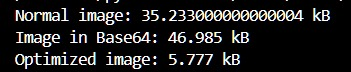
\includegraphics[width=0.5\linewidth]{Hauptkapitel/Pictures/opt_img.jpg}
    \caption{File size comparison}
    \label{fig:opt_img}
\end{figure}
The following code belongs to the function that automates the processes involved in the picture capturing and its optimization for publishing.

\begin{lstlisting}[style=courier12]
def publish_photo(client):
    """Captures and publishes a photo as base64 data MQTT message."""
    try:
        os.system("libcamera-jpeg --output \"test.jpg\" --width 640 --height 480 -n")
        foo = Image.open("test.jpg")
        foo.save('optimizedtest.jpg', optimize=True, quality=40)
        with open("optimizedtest.jpg", "rb") as image_file:
          image = image_file.read()
        print(f"Read {len(image)} bytes")
        client.publish(TOPIC_PHOTO, image, qos=2)
        print("Photo successfully sent.")
    except FileNotFoundError:
        print("[ERROR] test.jpg not found.")
    except Exception as e:
        print(f"[ERROR] Failed to publish photo: {e}")
\end{lstlisting}



 



 

